% =====================================================================
%  Introduction to Deep Learning — Class 9
%  Topic (course plan): Deep Networks
%  Subtopics (course plan): MLP/FNN to Universal Function Approximation,
%                           Depth and Width efficiency, Theorems
%  Sources (course plan): Bishop Chapter 6, Prince Chapter 4, publications
%
%  Figures: published figures from Bishop & Bishop (2024) Ch. 6 and
%  Prince (2023) Ch. 4, reproduced with attribution.  The plots that
%  illustrate published *rates* (Barron, Telgarsky, Montufar, Bartlett)
%  have no textbook counterpart and are generated -- see
%  ../B_Recreated_Figures/src/.
%  Notation: the fixed course convention (see _shared/NOTATION.md).
%
%  Compile:  xelatex main.tex   (run twice)
% =====================================================================
\documentclass[aspectratio=169, 11pt]{beamer}

\usetheme{metropoliscustom}

\usepackage{graphicx}
\DeclareGraphicsExtensions{.pdf,.png,.jpg}
\graphicspath{{figs_official/}{Class09_MLP_Universal_Approximation_Efficiency/A_Textbook_Figures/figs_official/}}
\usepackage{amsmath, amssymb}
\usepackage{bm}
\usepackage{tikz}
\usetikzlibrary{arrows.meta, positioning, calc, decorations.pathreplacing}
\tcbuselibrary{skins}

\definecolor{shc}{HTML}{341651}
\definecolor{tealc}{HTML}{1C7293}
\definecolor{dpc}{HTML}{800000}
\definecolor{accc}{HTML}{B8860B}

% ---- theorem environments -------------------------------------------
\setbeamertemplate{theorems}[numbered]
\newtheorem{lemmax}[theorem]{Lemma}
\newtheorem{propx}[theorem]{Proposition}
\newtheorem{corx}[theorem]{Corollary}

% ---- parallel strip: Shallow (left) vs Deep (right) ------------------
\newcommand{\shpar}[2]{%
  \vfill
  {\scriptsize
  \begin{tcolorbox}[enhanced, sidebyside, sidebyside align=top,
                    lefthand ratio=0.485,
                    segmentation style={shc!35, line width=0.6pt},
                    colback=shc!5, colframe=shc!35, boxrule=0.5pt,
                    arc=1.2mm, left=1.6mm, right=1.6mm,
                    top=0.6mm, bottom=0.6mm,
                    before skip=0pt, after skip=0pt]
    {\color{shc}\textbf{SHALLOW}}\hspace{0.55em}#1
  \tcblower
    {\color{dpc}\textbf{DEEP}}\hspace{0.55em}#2
  \end{tcolorbox}}%
  \vspace{0.35em}%
}

% ---- a one-line lead-in that says why this slide follows the last --
\newcommand{\bridge}[1]{%
  {\scriptsize\itshape\color{mcMuted} #1\par}\vspace{0.35em}}

\newcommand{\figsource}[1]{{\scriptsize\color{mcMuted} #1}}
\newcommand{\figcap}[2][0.90]{%
  \begin{center}\begin{minipage}{#1\textwidth}\centering
    {\scriptsize\color{mcMuted} #2}
  \end{minipage}\end{center}}

\newcommand{\unit}[4]{%
  \node[circle, draw=#3, fill=#3!6, line width=0.7pt,
        minimum size=10mm, inner sep=0pt] (#1) at #2 {};
  \begin{scope}
    \clip #2 circle (0.5);
    \draw[tealc, line width=1.1pt]
      ($#2+(-0.50,-0.26)$) -- ($#2+(0.02,-0.26)$) -- ($#2+(0.46,0.28)$);
  \end{scope}
  \node[font=\large, #3] at ($#2+(0,0.78)$) {#4};
}
\newcommand{\plainunit}[4]{%
  \node[circle, draw=#3, fill=black!4, line width=0.7pt,
        minimum size=10mm, inner sep=0pt, font=\small] (#1) at #2 {#4};
}

% =====================================================================
\title{Deep Networks}
\subtitle{MLP/FNN to Universal Function Approximation, Depth and Width
          Efficiency}
\author{Introduction to Deep Learning \ \textperiodcentered\ Class 9}
\institute{}
\date{10 August}

\footleft{Introduction to Deep Learning}
\footright{Depth and Width Efficiency}
\titlelogos{}

\begin{document}

\maketitle

\begin{frame}{Outline}
  \tableofcontents
\end{frame}

% =====================================================================
\section{The Multilayer Perceptron, Formally}
% =====================================================================

\begin{frame}{Notation used throughout this course}
  \vspace{0.2em}
  {\footnotesize
  \renewcommand{\arraystretch}{1.22}
  \begin{columns}[T, onlytextwidth]
    \begin{column}{0.49\textwidth}
      \begin{tabular}{@{}l@{\hspace{1.5em}}l@{}}
        $\mathbf{x}\in\mathbb{R}^{D}$ & input / \alert{features}\\
        $y$, $\hat y$ & target, model \alert{prediction}\\
        $\mathbf{z}^{(l)}=h(\mathbf{a}^{(l)})$ & units of hidden layer $l$\\
        $\mathbf{W}^{(l)}$, $\mathbf{b}^{(l)}$ & weights and biases\\
        $L$, $M$ & \alert{depth}, \alert{width}\\
        $W$ & total number of parameters\\
      \end{tabular}
    \end{column}
    \begin{column}{0.49\textwidth}
      \begin{tabular}{@{}l@{\hspace{1.5em}}l@{}}
        $\phi_j(\mathbf{x})$ & \alert{fixed} basis function\\
        $\mathcal{K}\subset\mathbb{R}^{D}$ & a compact set\\
        $C(\mathcal{K})$ & continuous functions on $\mathcal{K}$\\
        $\lVert f\rVert_\infty$ & $\sup_{\mathbf{x}\in\mathcal{K}}|f(\mathbf{x})|$\\
        $\varepsilon$ & target accuracy\\
        $\mathcal{N}_{L,M}$ & functions a network can compute\\
      \end{tabular}
    \end{column}
  \end{columns}}
  \vfill
  \begin{redhighlight}
    {\footnotesize Symbols follow \textbf{Bishop \& Bishop (2024)}.
    $W$ counts every weight and bias; $\mathcal{N}_{L,M}$ is the set of
    functions a network of that shape can compute.}
  \end{redhighlight}
\end{frame}

\begin{frame}{Where Class 7 left us}
  \vspace{0.3em}
  \begin{itemize}\setlength{\itemsep}{4pt}
    \item Composition \alert{multiplies} linear pieces; width only
          \alert{adds} them
    \item Universal approximation holds in $D$ dimensions for any
          non-polynomial activation, via ridge functions
    \item ReLU networks compute \alert{exactly} the continuous
          piecewise-linear functions --- shallow or deep
    \item The sawtooth needs $O(L)$ units deep and $2^{L}-1$ shallow
  \end{itemize}
  \vspace{0.4em}
  \begin{redhighlight}
    All of that was about \alert{what} a network can represent. None of
    it says \alert{how much network} it takes.
  \end{redhighlight}
\end{frame}

\begin{frame}{Three questions, and where they are answered}
  \vspace{0.2em}
  \centering
  \renewcommand{\arraystretch}{1.35}
  {\small
  \begin{tabular}{p{0.05\textwidth} p{0.40\textwidth}
                  p{0.42\textwidth}}
    & \textbf{Question} & \textbf{Answered by}\\
    \hline
    1 & Can one hidden layer reach any function at all?
      & Cybenko, Hornik, Leshno \hfill{\scriptsize \S2}\\
    2 & How fast does the error fall as the network grows?
      & Barron; DeVore et al. \hfill{\scriptsize \S2}\\
    3 & How much of the budget should be width, and how much depth?
      & Lu et al.; Telgarsky; Eldan \& Shamir; Yarotsky
        \hfill{\scriptsize \S3--4}\\
    \hline
  \end{tabular}}
  \vspace{0.7em}

  {\small A fourth question follows from the third: if depth buys so
  much expressive power, what does that power \alert{cost} in data?
  That is \S5.}
\end{frame}

\begin{frame}{The multilayer perceptron}
  \bridge{Before we can count anything, we need to fix exactly what we
  are counting.}
  \begin{columns}[T, onlytextwidth]
    \begin{column}{0.46\textwidth}
      \centering
      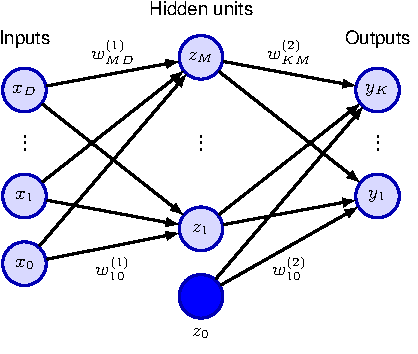
\includegraphics[height=0.255\textheight]{Bishop6_9}
      \\[0.1em]
      \figsource{Figure from Bishop \& Bishop (2024), Fig.~6.9.}
    \end{column}
    \hfill
    \begin{column}{0.50\textwidth}
      \centering
      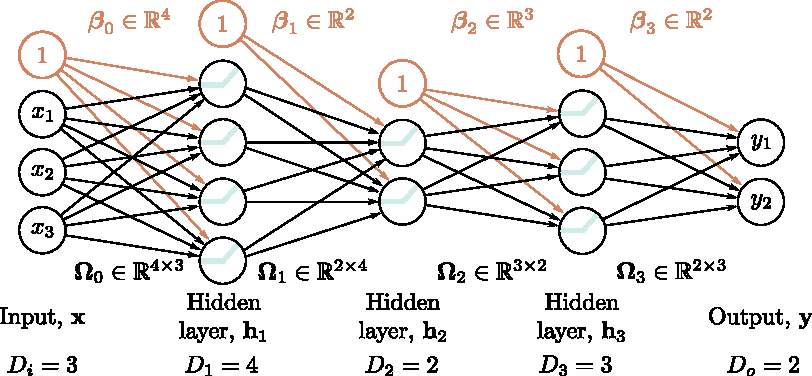
\includegraphics[height=0.255\textheight]{DeepKLayer}
      \\[0.1em]
      \figsource{Figure from Prince (2023), Fig.~4.6: the same network
      with $L$ hidden layers and their dimensions.}
    \end{column}
  \end{columns}
  \vspace{0.2em}
  \[
    \mathbf{z}^{(0)}=\mathbf{x},
    \qquad
    \mathbf{z}^{(l)} = h\big(\mathbf{W}^{(l)}\mathbf{z}^{(l-1)}
    + \mathbf{b}^{(l)}\big),
    \qquad
    \hat y = \mathbf{W}^{(L+1)}\mathbf{z}^{(L)} + b^{(L+1)}
  \]
  \vspace{-0.5em}
  {\scriptsize $\mathcal{N}_{L,M}$ denotes the functions this computes,
  with $W = M(D{+}1) + (L{-}1)M(M{+}1) + (M{+}1)$ parameters.}
\end{frame}

\begin{frame}{Why not just use fixed basis functions?}
  \bridge{Before calling learned features progress, see what goes
  wrong without them.}
  Tile the input space, one basis function per cell
  (B\&B, 2024, \S6.1):
  \[
    \hat y(\mathbf{x}) = \sum_{j} w_j\,\phi_j(\mathbf{x}),
    \qquad
    \phi_j \text{ centred on cell } j
  \]
  \vspace{0.05em}
  \begin{propx}[The grid blows up]
    {\small Partition each of the $D$ axes into $S$ intervals. The
    tensor-product grid then has \alert{$S^{D}$} cells, so the model has
    $S^{D}$ parameters --- exponential in the input dimension.}
  \end{propx}
  \vspace{-0.05em}
  {\footnotesize
  \emph{Proof.} A cell is one interval chosen per axis, so there are
  $|\{1,\dots,S\}^{D}| = S^{D}$. \hfill$\square$}

  \vspace{0.7em}
  {\footnotesize With $S=10$ and a $32\times32$ image ($D=1024$):
  $10^{1024}$ cells.}
\end{frame}

\begin{frame}{The curse of dimensionality, drawn}
  \vspace{0.3em}
  \begin{columns}[c, onlytextwidth]
    \begin{column}{0.30\textwidth}\centering
      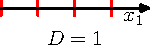
\includegraphics[width=0.92\linewidth]{Bishop6_3a}
    \end{column}
    \begin{column}{0.30\textwidth}\centering
      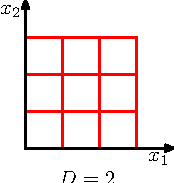
\includegraphics[width=0.72\linewidth]{Bishop6_3b}
    \end{column}
    \begin{column}{0.30\textwidth}\centering
      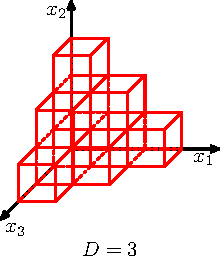
\includegraphics[width=0.82\linewidth]{Bishop6_3c}
    \end{column}
  \end{columns}
  \vspace{0.4em}
  \figcap[0.96]{Figure from Bishop \& Bishop (2024), Fig.~6.3: a regular
  grid over the input space in $D=1$, $2$ and $3$. The number of cells
  grows as $S^{D}$, so each extra input dimension multiplies the number
  of parameters.}
  \vspace{-0.1em}
  {\footnotesize Every cell needs its own parameter --- and its own
  data to fit it.}
\end{frame}

\begin{frame}{Two more faces of the same problem}
  \bridge{High-dimensional space is strange in two further ways that
  matter later.}
  \begin{center}
    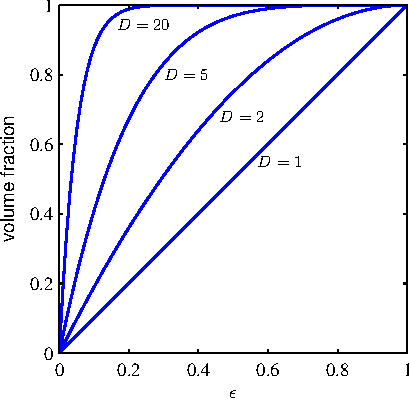
\includegraphics[height=0.285\textheight]{Bishop6_4}\hspace{1.8em}
    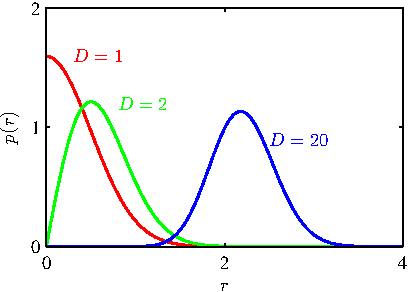
\includegraphics[height=0.285\textheight]{Bishop6_5}
  \end{center}
  \figcap[0.96]{Figures from Bishop \& Bishop (2024), Figs.~6.4 and 6.5.
  Left: the volume of a sphere lying in an outer shell of thickness
  $\epsilon$. Right: a Gaussian's radial density, whose mass migrates to
  a shell at radius $\approx\sqrt{D}$.}
  \shpar{fixed $\phi_j$: one parameter per cell, $S^{D}$ of them}
        {learned features: units \emph{move} to where the data is}
\end{frame}

% =====================================================================
\section{Universal Approximation, Revisited}
% =====================================================================

\begin{frame}{What ``universal'' means}
  \bridge{Networks are supposed to escape this. First, say precisely
  what that claim asserts.}
  Fix a compact $\mathcal{K}\subset\mathbb{R}^{D}$ and use the supremum
  norm $\lVert f\rVert_\infty=\sup_{\mathbf{x}\in\mathcal{K}}
  |f(\mathbf{x})|$.
  \vfill
  \begin{block}{Definition}
    {\small A family $\mathcal{F}\subset C(\mathcal{K})$ is
    \alert{universal} (dense) if for every $f\in C(\mathcal{K})$ and
    every $\varepsilon>0$ there is $g\in\mathcal{F}$ with
    $\lVert f-g\rVert_\infty<\varepsilon$.}
  \end{block}
  \vfill
  {\small
  \begin{itemize}\setlength{\itemsep}{3pt}
    \item Note what is quantified: $\mathcal{F}$ is the family with
          \alert{unbounded} width, so ``$g$ exists'' may mean a network
          of astronomical size
    \item Density says nothing about \alert{how fast} the error falls
          as the network grows --- that needs a \alert{rate}
  \end{itemize}}
\end{frame}

\begin{frame}{The classical statement}
  \bridge{With the definition in place, the theorem is short.}
  \begin{theorem}[Universal approximation; Cybenko 1989, Hornik 1991,
                  Leshno et al.\ 1993]
    {\small Let $h:\mathbb{R}\to\mathbb{R}$ be continuous. The family
    \[
      \mathcal{N}_{1,\infty}
      = \Big\{\,\mathbf{x}\mapsto \sum_{j=1}^{M} w^{(2)}_j\,
        h\big(\mathbf{w}_j^{(1)\top}\mathbf{x}+w^{(1)}_{j0}\big)
        + w^{(2)}_0 \;:\; M\in\mathbb{N} \Big\}
    \]
    is dense in $C(\mathcal{K})$ for every compact $\mathcal{K}$
    \alert{if and only if $h$ is not a polynomial}.}
  \end{theorem}
  \vspace{0.1em}
  {\footnotesize
  \begin{itemize}\setlength{\itemsep}{2pt}
    \item Proved in Class 7 by reduction to one dimension through
          \alert{ridge functions}
    \item \alert{One hidden layer is enough} --- so universality alone
          can never be an argument for depth
  \end{itemize}}
\end{frame}

\begin{frame}{Universal approximation, illustrated}
  \begin{center}
    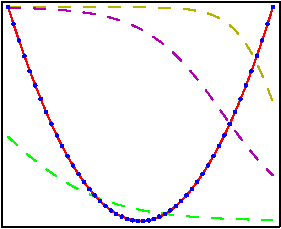
\includegraphics[height=0.235\textheight]{Bishop6_10a}\hspace{0.6em}
    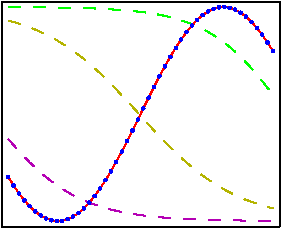
\includegraphics[height=0.235\textheight]{Bishop6_10b}\hspace{0.6em}
    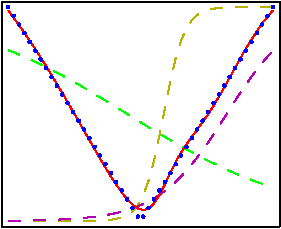
\includegraphics[height=0.235\textheight]{Bishop6_10c}\hspace{0.6em}
    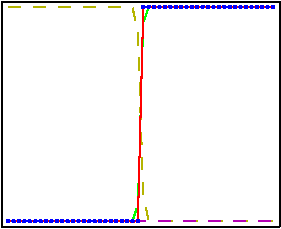
\includegraphics[height=0.235\textheight]{Bishop6_10d}
  \end{center}
  \figcap[0.97]{Figure from Bishop \& Bishop (2024), Fig.~6.10: one
  two-layer network with three $\tanh$ hidden units, fitted to
  $x^{2}$, $\sin(2\pi x)$, $|x|$ and the step $\mathbb{1}[x>0]$.
  Dashed are the individual hidden-unit contributions; solid is the
  network output.}
  \vspace{0.2em}
  {\footnotesize
  \begin{itemize}\setlength{\itemsep}{1pt}
    \item Even three units get close; the theorem says the error goes
          to zero as the width grows
    \item The step function shows the limit: a continuous network can
          only approximate a discontinuity, never match it
  \end{itemize}}
\end{frame}

\begin{frame}{Two objects the next two theorems need}
  \vspace{0.1em}
  \bridge{Density says the error reaches zero. To ask \emph{how fast},
  we must first say which functions we mean.}
  \begin{columns}[T, onlytextwidth]
    \begin{column}{0.485\textwidth}
      \begin{block}{The Barron norm}
        {\scriptsize
        \[ C_f=\int \lVert\bm\omega\rVert\,
           \big|\tilde f(\bm\omega)\big|\,\mathrm{d}\bm\omega \]
        $\tilde f(\bm\omega)$ is the Fourier transform: how much of $f$
        sits at frequency $\bm\omega$. Weighting by
        $\lVert\bm\omega\rVert$ \alert{charges a function for its
        high-frequency content}.}
      \end{block}

    \end{column}
    \hfill
    \begin{column}{0.485\textwidth}
      \begin{block}{A smoothness ball}
        {\scriptsize
        \[ \mathcal{F}=\big\{f:\ \lVert \partial^{\alpha}f
           \rVert_\infty\leq 1 \ \ \forall\,|\alpha|\leq s\big\} \]
        Every derivative up to order $s$ is bounded by one. This is the
        Sobolev ball $W^{s,\infty}$: \alert{all functions of a given
        smoothness, taken together}.}
      \end{block}

    \end{column}
  \end{columns}
  \vspace{-0.1em}
  \begin{redhighlight}
    {\footnotesize One measures a \alert{single} function's
    wiggliness, the other a \alert{whole class} --- which is why the two
    bounds point opposite ways. A bound over a ball is worst-case.}
  \end{redhighlight}
\end{frame}

\begin{frame}{A rate that does not see the dimension}
  \bridge{Take a function with small $C_f$. How quickly does a
  one-hidden-layer network close in on it?}
  \begin{theorem}[Barron, 1993]
    {\small Let $f:\mathcal{K}\to\mathbb{R}$ have finite Barron norm
    $C_f<\infty$. Then for every $M$ there is a
    one-hidden-layer sigmoidal network $\hat y_M$ with $M$ units and
    \[
      \int_{\mathcal{K}}\big(f(\mathbf{x})-\hat y_M(\mathbf{x})\big)^2
      \,\mu(\mathrm{d}\mathbf{x})
      \;\leq\; \frac{(2C_f r)^2}{M},
    \]
    with $r$ the radius of $\mathcal{K}$. The bound is
    \alert{independent of $D$}.}
  \end{theorem}
  \vspace{-0.2em}
  {\scriptsize
  \begin{itemize}\setlength{\itemsep}{0pt}
    \item \focus{1}{\emph{Proof sketch.} Write $f$ as a continuous
          mixture of ridge functions, with total mass controlled by
          $C_f$}
    \item \focus{2}{So $f$ is in the \alert{closed convex hull} of
          scaled ridge functions of norm $\leq 2C_f r$}
    \item \focus{3}{Maurey's lemma: a point of the convex hull of
          norm-$b$ elements lies within $b/\sqrt{M}$ of an average of
          $M$ of them}
    \item \focus{4}{That average \emph{is} an $M$-unit network
          \hfill $\square$}
  \end{itemize}}
\end{frame}

\begin{frame}{The rate, measured}
  \begin{columns}[T, onlytextwidth]
    \begin{column}{0.53\textwidth}
      \centering
      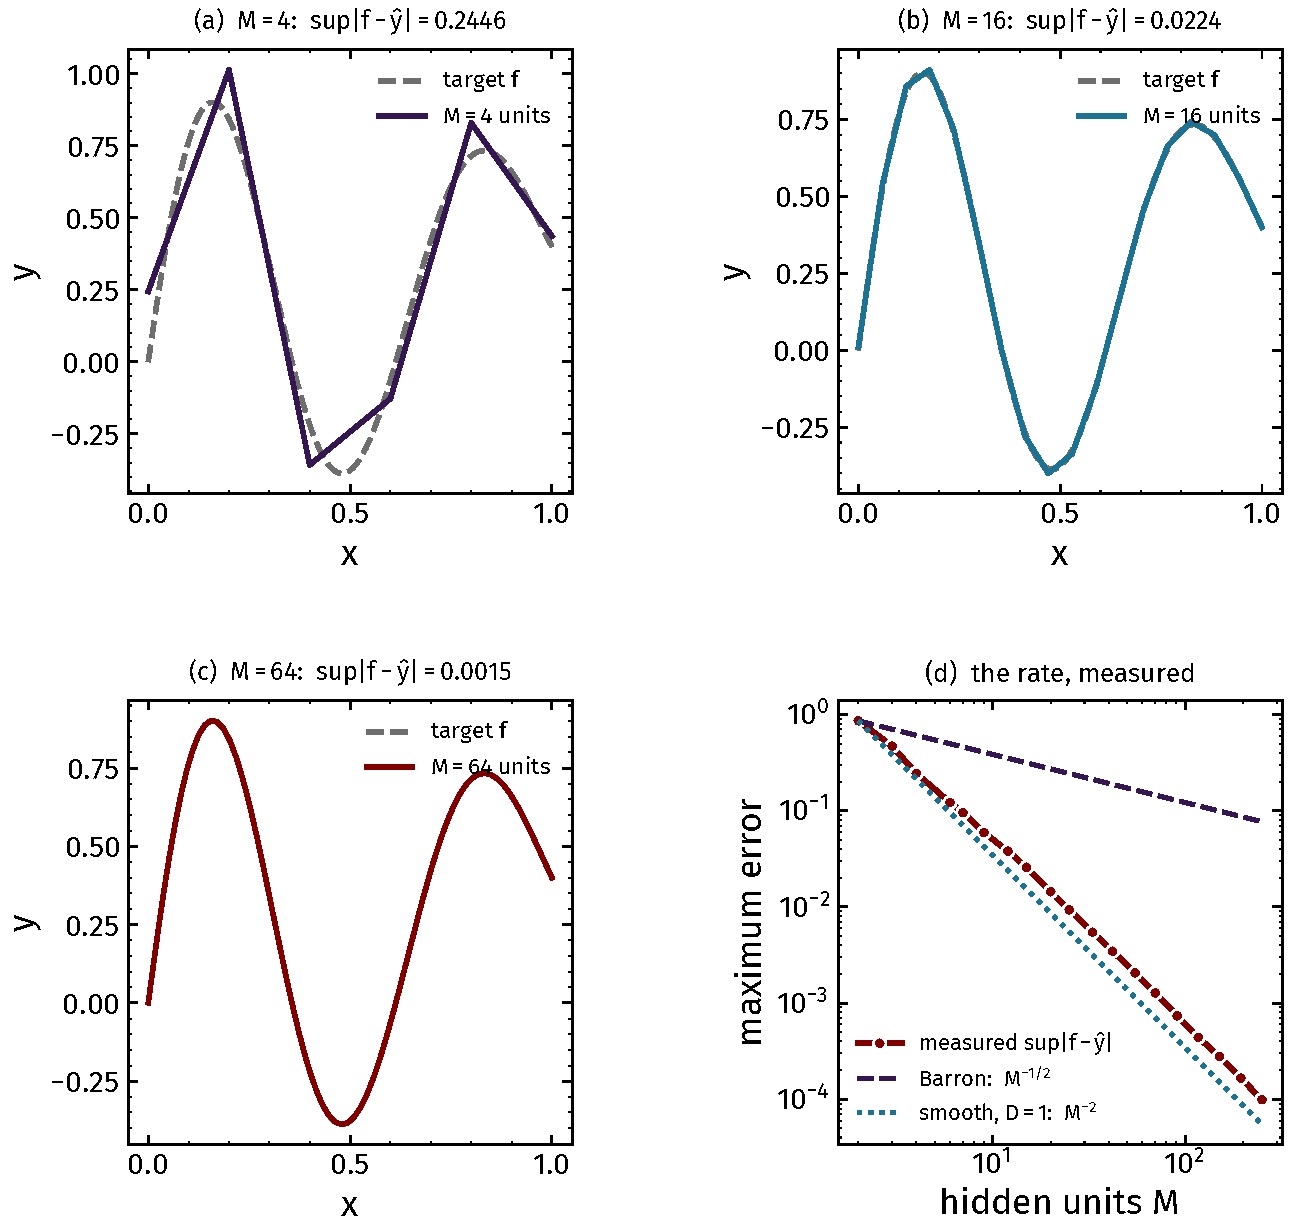
\includegraphics[height=0.72\textheight]{uat_rate}
    \end{column}
    \hfill
    \begin{column}{0.43\textwidth}
      \vspace{0.6em}
      {\small
      \begin{itemize}\setlength{\itemsep}{5pt}
        \item (a--c) the best $M$-unit fit to one smooth target as $M$
              grows
        \item (d) the measured error against two references
        \item Barron's $M^{-1/2}$ is a \alert{worst-case guarantee}
              over a whole class; a single smooth target in $D=1$ does
              much better, here $M^{-2}$
        \item A theorem gives a ceiling on the error, not a
              prediction of it
      \end{itemize}}
    \end{column}
  \end{columns}
\end{frame}

\begin{frame}{And a lower bound that does}
  \bridge{Barron's class is generous to us. What happens if we ask for a
  guarantee over \emph{all} functions of a given smoothness instead?}
  \begin{theorem}[DeVore, Howard \& Micchelli, 1989]
    {\small Let $\mathcal{F}$ be the unit ball of the Sobolev space
    $W^{s,\infty}([0,1]^{D})$. If an approximation scheme uses $W$
    parameters chosen \alert{continuously} from the target, then its
    worst-case error over $\mathcal{F}$ is at least
    $c\,W^{-s/D}$.}
  \end{theorem}
  \vspace{0.1em}
  {\scriptsize
  \begin{itemize}\setlength{\itemsep}{2pt}
    \item Smoothness $s$ buys accuracy; dimension $D$ takes it away.
          To halve the error in $D$ dimensions you need
          $2^{D/s}$ times the parameters
    \item It limits \alert{every} scheme with continuous parameter
          selection, not networks in particular
    \item No contradiction with Barron: his class is \alert{much
          smaller} than a Sobolev ball
  \end{itemize}}
  \vspace{-0.1em}
  \begin{redhighlight}
    {\scriptsize The curse is real. It is escaped only by targets with
    extra structure --- which is exactly what real data has.}
  \end{redhighlight}
\end{frame}

\begin{frame}{The two bounds side by side}
  \begin{center}
    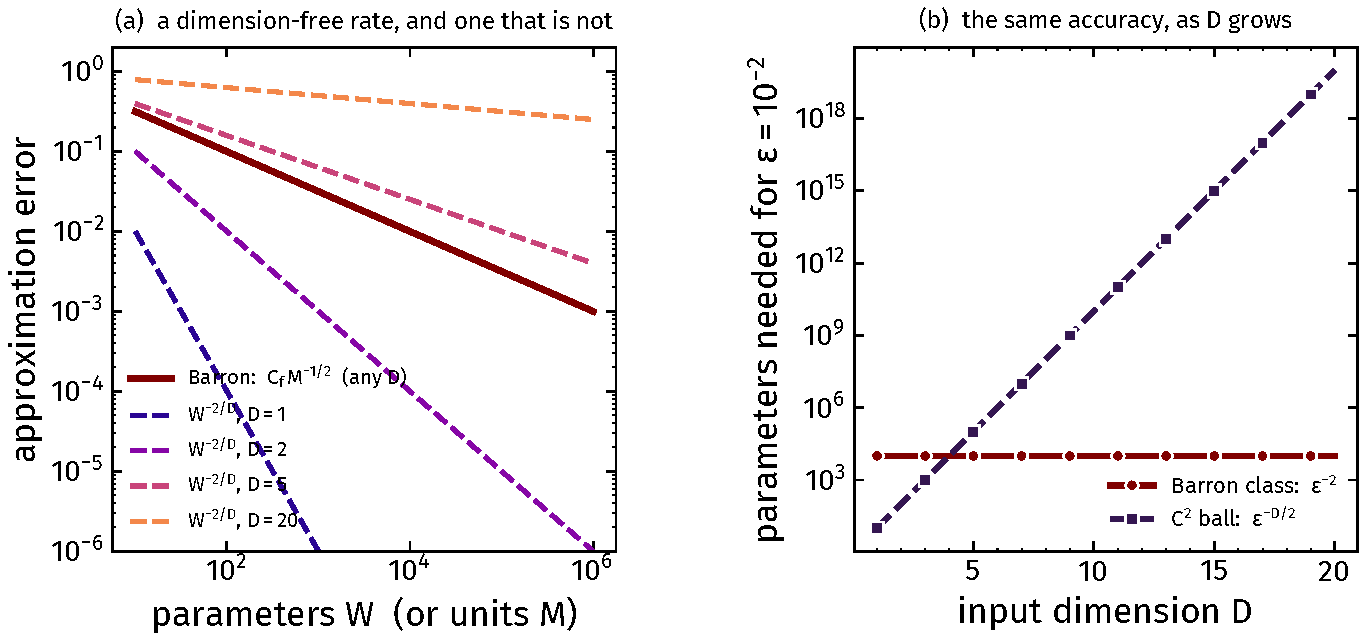
\includegraphics[height=0.505\textheight]{barron_vs_curse}
  \end{center}
  \figcap[0.96]{(a) the dimension-free Barron rate against the Sobolev
  lower bound for several $D$: for $D=1$ or $2$ smoothness wins, but by
  $D=20$ the Barron bound is far better. (b) parameters needed for
  $\varepsilon=10^{-2}$: constant in the Barron class, exponential in
  $D$ on a $C^{2}$ ball.}
\end{frame}

% =====================================================================
\section{How Wide Must a Network Be?}
% =====================================================================

\begin{frame}{Width as a threshold: the upper bound}
  \bridge{We know the cost of accuracy. Now: how to spend the budget.
  Width behaves quite unlike depth.}
  \vspace{0.3em}
  \begin{theorem}[Width-bounded universality; Lu, Pu, Wang, Hu \& Wang,
                  2017]
    {\small ReLU networks of width $D+4$ and \alert{arbitrary depth} are
    dense in $L^{1}(\mathbb{R}^{D})$: for every Lebesgue-integrable $f$
    and every $\varepsilon>0$ there is such a network with
    $\int|f-\hat y|\,\mathrm{d}\mathbf{x}<\varepsilon$.}
  \end{theorem}
  \vspace{0.5em}
  {\small
  \begin{itemize}\setlength{\itemsep}{4pt}
    \item Four units more than the input dimension is \alert{all} the
          width that is ever needed, provided the network may be deep
    \item Note the norm: density in $L^{1}$, not uniform
          approximation
  \end{itemize}}
\end{frame}

\begin{frame}{Width as a threshold: the lower bound}
  \bridge{Four units of slack sounds arbitrary. It is not --- just below
  it, everything fails.}
  \vspace{0.2em}
  \begin{theorem}[Width lower bound; Hanin \& Sellke 2017, Johnson 2019]
    {\small ReLU networks of width \alert{$\leq D$} are \emph{not}
    universal, however deep. There are continuous functions they cannot
    approximate to better than a fixed constant.}
  \end{theorem}
  \vspace{0.3em}
  {\small
  \emph{Why it holds.} A ReLU network of width $\leq D$ never expands
  the space it maps through, so all of its \alert{level sets are
  unbounded}. A function with a bounded level set --- say
  $\lVert\mathbf{x}\rVert$, whose level sets are spheres --- cannot be
  approximated.}
  \vspace{0.25em}
  \begin{redhighlight}
    {\small \alert{Width is a threshold}: below $D$ nothing works, just
    above it everything does. \alert{Depth is a resource}.}
  \end{redhighlight}
\end{frame}

% =====================================================================
\section{How Much Does Depth Buy?}
% =====================================================================

\begin{frame}{The witness, recalled}
  \bridge{Width has a floor and then stops mattering. Depth has no such
  ceiling.}
  \vspace{0.4em}
  \begin{lemmax}[The sawtooth, from Class 7]
    {\small $T(x)=2h(x)-4h(x-\tfrac12)$ is a two-unit ReLU network that
    maps $[0,1]$ onto $[0,1]$, folding it in half. Its $L$-fold
    composition $T^{\circ L}$ has exactly $2^{L}$ linear pieces and is
    computed by a network of depth $L$ and width $2$.}
  \end{lemmax}
  \vspace{0.5em}
  {\small Two units per layer, $L$ layers --- and the number of pieces
  \alert{doubles with every layer added}. That is the whole mechanism.}
\end{frame}

\begin{frame}{Depth beats width, provably}
  \vspace{0.3em}
  \begin{theorem}[Depth--width separation; Telgarsky, 2016]
    {\small $T^{\circ L}$ is computed by a ReLU network with $O(L)$
    parameters, but any \alert{one-hidden-layer} ReLU network computing
    it exactly needs at least $2^{L}-1$ units. Telgarsky's full result
    strengthens ``exactly'' to ``to within a constant''.}
  \end{theorem}
  \vspace{0.4em}
  {\small
  \emph{Proof of the lower bound.} A one-hidden-layer ReLU network with
  $M$ units on a scalar input is piecewise linear with at most $M+1$
  pieces. Matching $2^{L}$ pieces forces $M+1\geq 2^{L}$.
  \hfill$\square$}
  \vspace{0.4em}
  \begin{redhighlight}
    {\small An \alert{exponential} gap, from a function you can draw in
    one line.}
  \end{redhighlight}
\end{frame}

\begin{frame}{The separation, measured}
  \vspace{-0.6em}
  \begin{center}
    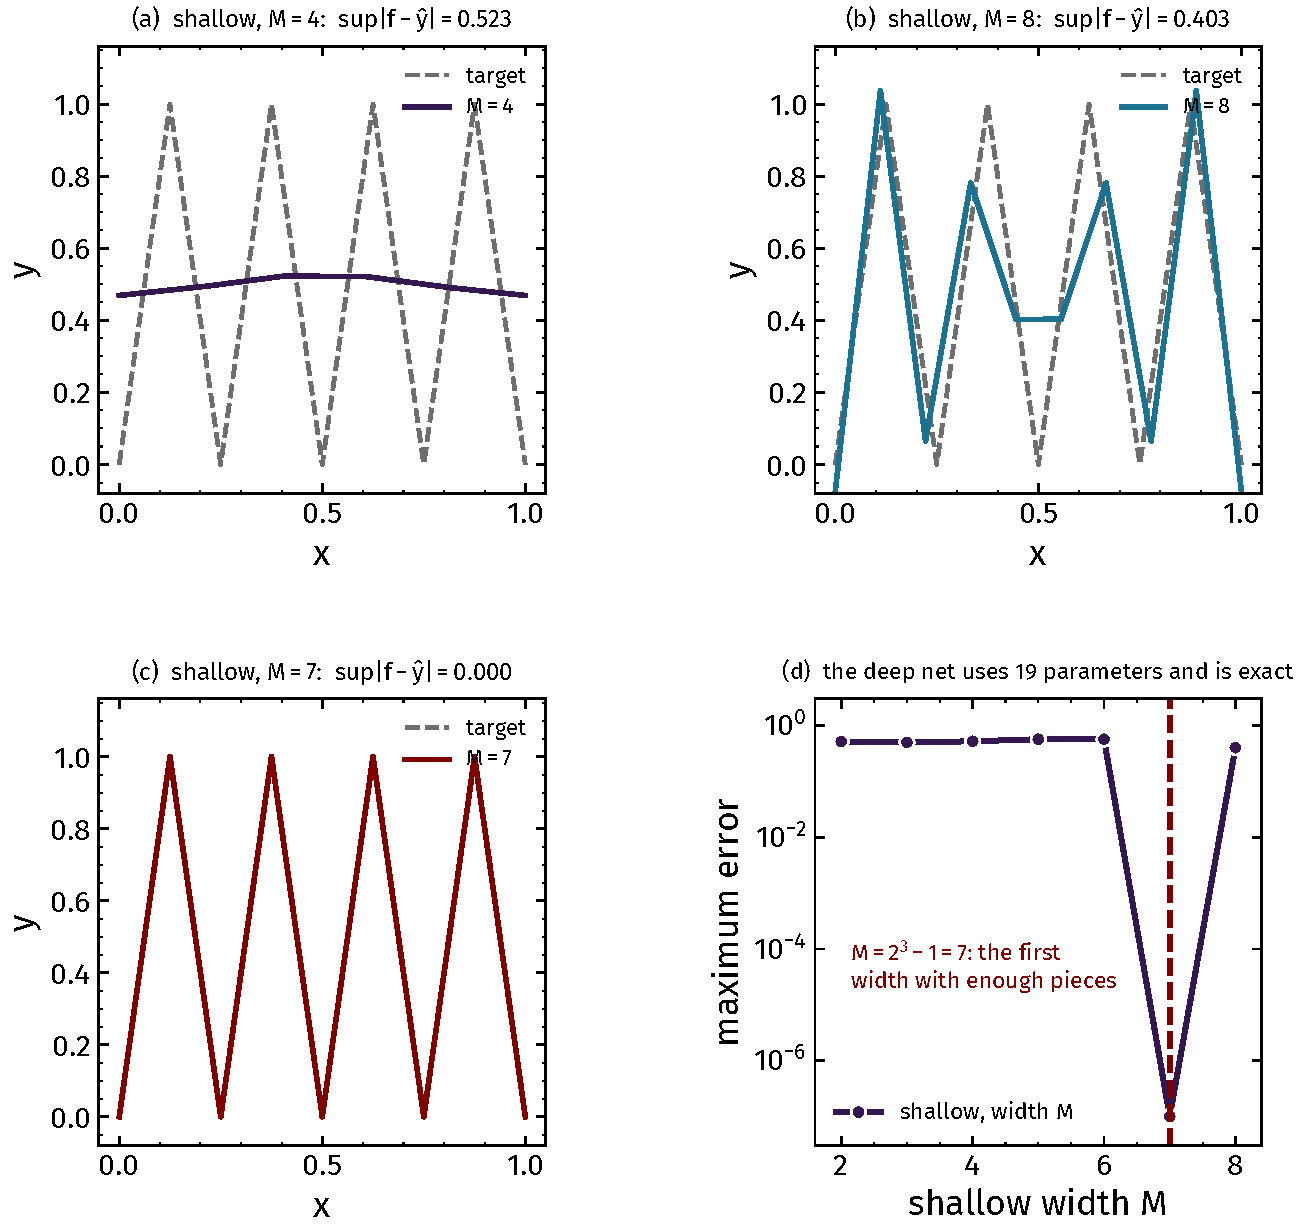
\includegraphics[height=0.735\textheight]{depth_width}
  \end{center}
\end{frame}

\begin{frame}{A separation that is not one-dimensional}
  \bridge{The sawtooth lives on a line --- easy to dismiss. The same
  gap appears in $D$ dimensions.}
  \begin{theorem}[Eldan \& Shamir, 2016]
    {\small There is a \alert{radial} function
    $g:\mathbb{R}^{D}\to\mathbb{R}$, supported on a ball, that a network
    with \alert{three} layers and $\mathrm{poly}(D)$ width approximates
    to within a constant in $L^{2}$, but which \alert{every two-layer}
    network needs width $\exp(\Omega(D))$ to approximate that well.}
  \end{theorem}
  \vspace{0.1em}
  {\footnotesize
  \begin{itemize}\setlength{\itemsep}{2pt}
    \item Why radial functions are hard for two layers: a two-layer net
          is a sum of \alert{ridge} functions, each constant along
          $D-1$ directions, and building a sphere out of hyperplanes is
          expensive
    \item Three layers can first compute
          $\lVert\mathbf{x}\rVert^{2}=\sum_i x_i^{2}$ with $D$ cheap
          units, then apply a one-dimensional function to it
    \item Unlike Telgarsky's, this separation is about
          \alert{approximation in $L^{2}$}, not exact representation,
          and grows with the \alert{dimension} rather than the depth
  \end{itemize}}
\end{frame}

\begin{frame}{How deep networks beat the grid}
  \bridge{Separations show depth \emph{can} win. This says what it
  costs.}
  \begin{theorem}[Yarotsky, 2017]
    {\small For $f$ in the unit ball of $C^{n}([0,1]^{D})$ and any
    $\varepsilon\in(0,1)$ there is a ReLU network with
    \[
      \text{depth } O\big(\log(1/\varepsilon)\big)
      \quad\text{and}\quad
      W = O\big(\varepsilon^{-D/n}\log(1/\varepsilon)\big)
      \text{ parameters}
    \]
    such that $\lVert f-\hat y\rVert_\infty\leq\varepsilon$. Up to the
    logarithm this is \alert{optimal}.}
  \end{theorem}
  \vspace{-0.05em}
  {\footnotesize
  \begin{itemize}\setlength{\itemsep}{0pt}
    \item Deep ReLU networks approximate $x^{2}$, hence products, with
          $O(\log(1/\varepsilon))$ layers --- the sawtooth again
    \item Depth enters only \alert{logarithmically}; the
          $\varepsilon^{-D/n}$ is unavoidable
  \end{itemize}}
  \vspace{-0.1em}
  \begin{redhighlight}
    {\scriptsize Depth removes the \alert{overhead}, not the curse.}
  \end{redhighlight}
\end{frame}

% =====================================================================
\section{Counting Capacity}
% =====================================================================

\begin{frame}{Counting linear regions}
  \bridge{Rates are one currency; counting the pieces is another, and
  easier to compute.}
  \vspace{0.3em}
  \begin{theorem}[Lower bound; Mont\'ufar, Pascanu, Cho \& Bengio, 2014]
    {\small A ReLU network with $L$ hidden layers of width $M\geq D$ on
    $\mathbb{R}^{D}$ can realise at least
    \[
      \Big(\prod_{l=1}^{L-1}\big\lfloor M/D \big\rfloor^{D}\Big)
      \sum_{j=0}^{D}\binom{M}{j}
    \]
    linear regions.}
  \end{theorem}
  \vspace{0.3em}
  {\small The trailing $\sum_{j\leq D}\binom{M}{j}$ is the
  \alert{Zaslavsky count} from Class 5: the last layer behaves like a
  shallow network, and the product in front is what depth adds.}
\end{frame}

\begin{frame}{Counting linear regions: the ceiling}
  \vspace{0.3em}
  \begin{theorem}[Upper bound; Serra, Tjandraatmadja \& Ramalingam, 2018]
    {\small The number of regions is at most
    $\prod_{l=1}^{L}\sum_{j=0}^{D}\binom{M}{j}$, and tighter bounds
    follow from the dimensions of the individual layers.}
  \end{theorem}
  \vspace{0.5em}
  {\small
  \begin{itemize}\setlength{\itemsep}{4pt}
    \item Both bounds are \alert{exponential in $L$} and only
          \alert{polynomial in $M$} --- the same asymmetry as the
          sawtooth
    \item A lower bound says such networks \alert{exist}; it does not
          say training finds them
  \end{itemize}}
\end{frame}

\begin{frame}{Regions against parameters}
  \begin{center}
    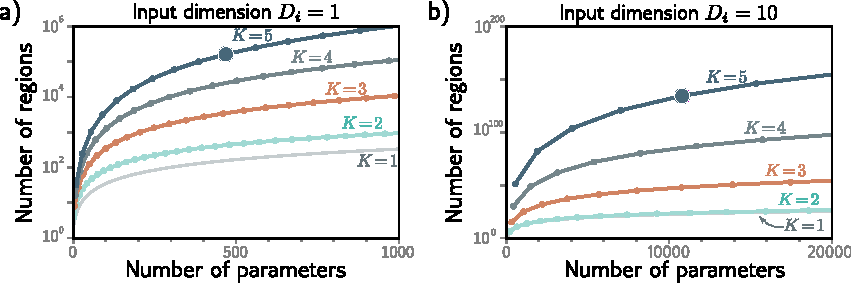
\includegraphics[height=0.47\textheight]{DeepParams}
  \end{center}
  \figcap[0.96]{Figure from Prince (2023), Fig.~4.9: the number of
  linear regions against the number of parameters, for (a) $D=1$ and
  (b) $D=10$ inputs, at several depths. Depth buys regions far faster
  than width does --- and the gap widens with the input dimension.}
\end{frame}

\begin{frame}{Capacity has a price}
  \bridge{Every result so far has been an argument for depth. Here is
  the bill.}
  \begin{theorem}[VC dimension; Bartlett, Harvey, Liaw \& Mehrabian, 2019]
    {\small For ReLU networks with $W$ parameters and $L$ layers,
    \[
      \mathrm{VCdim} \;=\; \Theta\big(W L \log W\big).
    \]}
  \end{theorem}
  \vspace{0.0em}
  {\footnotesize
  \begin{itemize}\setlength{\itemsep}{2pt}
    \item Learning theory then needs
          $N=\Omega(\mathrm{VCdim}/\epsilon^{2})$ samples for a gap
          $\epsilon$
    \item Modern networks have $\mathrm{VCdim}\gg N$ and generalise
          anyway: the bound is \alert{loose} for real data (Class 17)
  \end{itemize}}
  \vspace{-0.4em}
  \begin{redhighlight}
    {\scriptsize Expressivity and generalisation theorems pull in
    \alert{opposite directions}; neither alone explains deep learning.}
  \end{redhighlight}
\end{frame}

\begin{frame}{VC dimension, drawn}
  \begin{center}
    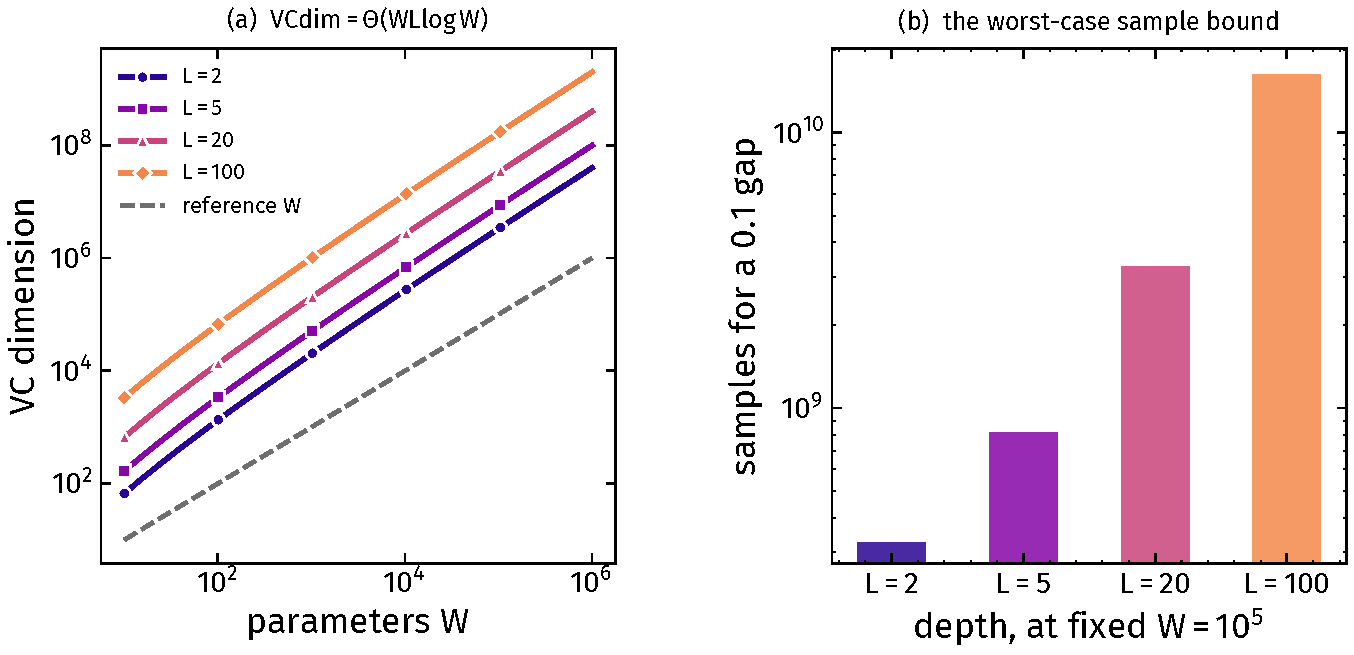
\includegraphics[height=0.505\textheight]{vc_growth}
  \end{center}
  \figcap[0.96]{(a) $\Theta(WL\log W)$ against the parameter count, at
  four depths, with a linear reference. (b) at a fixed $W=10^{5}$, the
  worst-case number of samples the VC bound demands for a
  generalisation gap of $0.1$ --- growing linearly with depth.}
\end{frame}

% =====================================================================
\section{Reading the Theorems}
% =====================================================================

\begin{frame}{What each theorem actually gives}
  \bridge{Ten results in one lecture. What each one is really claiming:}
  \centering
  \vspace{0.2em}
  \renewcommand{\arraystretch}{1.22}
  {\scriptsize
  \begin{tabular}{p{0.235\textwidth} p{0.30\textwidth}
                  p{0.36\textwidth}}
    \textbf{Result} & \textbf{Gives} & \textbf{Does not give}\\
    \hline
    Cybenko / Hornik / Leshno
      & density with one hidden layer, any non-polynomial $h$
      & any bound on the width\\
    Barron (1993)
      & $O(C_f/\sqrt{M})$, free of $D$
      & anything outside the Barron class; $C_f$ may grow with $D$\\
    DeVore et al.\ (1989)
      & $W^{-s/D}$ is unbeatable on a Sobolev ball
      & a statement about one particular target\\
    Lu et al.\ (2017)
      & width $D{+}4$ suffices, given depth
      & efficiency at that width\\
    Telgarsky (2016)
      & an explicit exponential depth gap
      & that such functions matter in practice\\
    Yarotsky (2017)
      & $O(\varepsilon^{-D/n}\log\frac{1}{\varepsilon})$, depth
        $O(\log\frac{1}{\varepsilon})$
      & escape from the curse\\
    Mont\'ufar (2014)
      & regions exponential in $L$
      & that training reaches them\\
    Bartlett et al.\ (2019)
      & $\mathrm{VCdim}=\Theta(WL\log W)$
      & a useful bound at modern scale\\
    \hline
  \end{tabular}}
\end{frame}

\begin{frame}{What none of them say}
  \bridge{And the gap between all this and a working network:}
  \vspace{0.2em}
  \begin{itemize}\setlength{\itemsep}{0pt}
    \item \alert{Nothing about optimisation.} Every result is about the
          \emph{existence} of weights; finding them is Classes 11--14
    \item \alert{Nothing about generalisation.} The capacity bounds
          are worst-case over all data distributions
    \item \alert{The hard cases may be irrelevant.} The sawtooth and
          the radial bump are built to be hard; natural signals are not
          adversarial
    \item \alert{Architecture matters more than the counts suggest.}
          Convolution and attention change the function class itself
  \end{itemize}
  \shpar{universal, but with a vacuous width bound}
        {universal \emph{and} efficient, on the functions we care about}
\end{frame}

\begin{frame}{Takeaways}
  \vspace{0.1em}
  {\footnotesize
  \begin{enumerate}\setlength{\itemsep}{2pt}
    \item Fixed basis functions need $S^{D}$ parameters. Networks avoid
          this by \alert{placing their features}, not tiling the space
    \item One hidden layer is already universal, for any
          non-polynomial activation --- so \alert{universality alone
          never argues for depth}
    \item Rates are what matter. \alert{Barron}: $O(C_f/\sqrt{M})$,
          free of dimension, on a restricted class.
          \alert{DeVore et al.}: $W^{-s/D}$ is unbeatable on a
          smoothness ball
    \item \alert{Width is a threshold} ($\leq D$ fails, $D+4$ suffices);
          \alert{depth is a resource} --- Telgarsky and Eldan--Shamir
          give explicit exponential gaps, and Yarotsky shows depth
          $O(\log\frac{1}{\varepsilon})$ removes the overhead
    \item Capacity counts both ways: regions grow exponentially in $L$,
          and so does the worst-case \alert{VC bound}
  \end{enumerate}}
  \vspace{-0.1em}
  \begin{redhighlight}
    {\scriptsize Class 11: having established what these networks can
    represent, how do we actually \alert{train} them?}
  \end{redhighlight}
\end{frame}

\begin{frame}{References}
  \scriptsize
  \begin{itemize}\setlength{\itemsep}{0pt}
    \item C.~M.~Bishop \& H.~Bishop. \textit{Deep Learning: Foundations
          and Concepts.} Springer, 2024. \S6.1 (limitations of fixed
          basis functions, the curse of dimensionality), \S6.2
          (multilayer networks), \S6.3 (deep networks).
    \item S.~J.~D.~Prince. \textit{Understanding Deep Learning.}
          MIT Press, 2023. Ch.~4 --- composition, folding, region
          counting, parameters versus regions.
    \item G.~Cybenko (1989); K.~Hornik (1991); M.~Leshno, V.~Lin,
          A.~Pinkus \& S.~Schocken, \textit{Neural Networks} 6:861
          (1993).
    \item A.~R.~Barron, \textit{IEEE Trans.\ Inf.\ Theory} 39:930
          (1993) --- dimension-free approximation rates.
    \item R.~DeVore, R.~Howard \& C.~Micchelli, \textit{Numer.\ Math.}
          63:469 (1989) --- nonlinear widths.
    \item Z.~Lu, H.~Pu, F.~Wang, Z.~Hu \& L.~Wang, \textit{NeurIPS}
          (2017); B.~Hanin \& M.~Sellke (2017); J.~Johnson,
          \textit{ICLR} (2019) --- width bounds.
    \item M.~Telgarsky, \textit{COLT} (2016); R.~Eldan \& O.~Shamir,
          \textit{COLT} (2016) --- depth separations.
    \item D.~Yarotsky, \textit{Neural Networks} 94:103 (2017) ---
          approximation rates for deep ReLU networks.
    \item G.~Mont\'ufar et al., \textit{NeurIPS} (2014); T.~Serra,
          C.~Tjandraatmadja \& S.~Ramalingam, \textit{ICML} (2018) ---
          linear regions.
    \item P.~Bartlett, N.~Harvey, C.~Liaw \& A.~Mehrabian,
          \textit{JMLR} 20:63 (2019) --- VC dimension.
    \item Figures 6.2--6.5, 6.9 and 6.10 reproduced from Bishop \&
          Bishop (2024); Figures 4.6 and 4.9 from Prince (2023),
          \url{https://udlbook.github.io/udlbook/}, CC BY-NC-ND.
          The rate and capacity plots have no textbook counterpart and
          are generated by
          \texttt{../B\_Recreated\_Figures/src/build\_all.py}.
  \end{itemize}
\end{frame}

\begin{frame}[standout]
  Questions?
\end{frame}

\end{document}
